\begin{questions}
\question
\begin{parts}
% question 1a
\part
* Suppose you have two parallel lines in 3-D space, one passing through the point$ (100,100,1000)$, the other through $(200,200,1100)$. The lines are parallel to the vector $(1,2,1)$. The lines are observed by a unit focal length camera at the origin (i.e. the camera reference frame and the world reference frame are identical). All coordinates are in camera coordinates. What is their point of intersection in the image? (Hint: the point of infinity along $\ell_i$ in 3-D space is given by $\lim_{\lambda_i\to\infty} \ell_i = \left(\begin{array}{c}X_i \\ Y_i \\ Z_i \\ \end{array} \right) + \lambda_i \left(\begin{array}{c}a \\ b \\ c \\ \end{array} \right)$, where $\left(\begin{array}{c}X_i \\ Y_i \\ Z_i \\ \end{array} \right)$ and $\left(\begin{array}{c}a \\ b \\ c \\ \end{array} \right)$ are a point on the line and its direction respectively)


\begin{solution}
  Denote the two parallel lines as follows:
  \[ \ell_a = \left(\begin{array}{c}100 \\ 100 \\ 1000 \\ \end{array} \right) + \lambda_a\left(\begin{array}{c}1 \\ 2 \\ 1 \\ \end{array} \right), \ell_b = \left(\begin{array}{c}200 \\ 200 \\ 1100 \\ \end{array} \right) + \lambda_b\left(\begin{array}{c}1 \\ 2 \\ 1 \\ \end{array} \right) \]
  
  Set $\lambda_a=100$ and $\lambda_a=200$ respectively to get two points on $\ell_a$:
  \[ P_{1a} = \left(\begin{array}{c}200 \\ 300 \\ 1100 \\ \end{array} \right), P_{2a} = \left(\begin{array}{c}300 \\ 500 \\ 1200 \\ \end{array} \right) \]
  
  Using the linear mapping of the perspective projection:
  
  \begin{equation}
  \left( \begin{array} { l } { x } \\ { y } \\ { w } \end{array} \right) = \left[ \begin{array} { c c c c } { f } & { 0 } & { 0 } & { 0 } \\ { 0 } & { f } & { 0 } & { 0 } \\ { 0 } & { 0 } & { 1 } & { 0 } \end{array} \right] \left( \begin{array} { c } { X _ { c } } \\ { Y _ { c } } \\ { Z _ { c } } \\ { 1 } \end{array} \right)
  \end{equation}
  
  The corresponding points (in $\mathcal{P}^2$) of $\mathbf{P}_{1a}$ and $\mathbf{P}_{2a}$ on the image are:
  \[ P^{'}_{1a} = \left[ \begin{array} { c c c c } { 1 } & { 0 } & { 0 } & { 0 } \\ { 0 } & { 1 } & { 0 } & { 0 } \\ { 0 } & { 0 } & { 1 } & { 0 } \end{array} \right] \left( \begin{array} { c } { 200 } \\ { 300 } \\ { 1100 } \\ { 1 } \end{array} \right) = \left(\begin{array}{c}200 \\ 300 \\ 1100 \\ \end{array} \right) \]
  
  \[ P^{'}_{2a} = \left[ \begin{array} { c c c c } { 1 } & { 0 } & { 0 } & { 0 } \\ { 0 } & { 1 } & { 0 } & { 0 } \\ { 0 } & { 0 } & { 1 } & { 0 } \end{array} \right] \left( \begin{array} { c } { 300 } \\ { 500 } \\ { 1200 } \\ { 1 } \end{array} \right) = \left(\begin{array}{c}300 \\ 500 \\ 1200 \\ \end{array} \right) \]
  
  The corresponding line (in $\mathcal{P}^2$) of $\ell_{a}$ on the image are formed by two points above:
  \[ \ell^{'}_a = P^{'}_{1a} \times P^{'}_{2a} = \left(\begin{array}{c}-190000 \\ 90000 \\ 10000 \\ \end{array} \right) \]
  
  Similarly, the corresponding line (in $\mathcal{P}^2$) of $\ell_{b}$ on the image can be obtained:
  \[ \ell^{'}_b = \left(\begin{array}{c}-200000 \\ 90000 \\ 20000 \\ \end{array} \right) \]
  
  Therefore, the intersection point (in $\mathcal{P}^2$) of the two parallel lines (in $\mathcal{N}^{3}$) on the image is:
  \[ P = \ell^{'}_a \times \ell^{'}_b  = \left(\begin{array}{c} 9 \times 10^{8} \\ 1.8 \times 10^{9} \\ 9 \times 10^{8} \\ \end{array} \right) \]
  
  Converting back to $\mathcal{N}^{2}$, $P = \left(\begin{array}{c} 1 \\ 2 \\ \end{array} \right)$ is the intersection point on the image.
  
\end{solution}

% question 1b
\part
Given the 3D coordinates of several corresponding points $P_i$ and $P_{i}^{'}$ in two views, you are required to find the 3D rotation $\mathbf{R}$ and translation $\mathbf{T}$ that relate the two views ($P_{i}^{'} = \mathbf{R}P_{i} + \mathbf{T}$). Formulate a linear least squares algorithm (of the form $\mathbf{A} \mathbf{x} = \mathbf{b}$) that ignores the orthogonality constraint associated with $\mathbf{R}$ (that is, it is okay if the solution for $\mathbf{R}$ returned by your formulation is not orthogonal). State the entries of the matrix $\mathbf{A}$, and the vectors $\mathbf{x}$ and $\mathbf{b}$.

\begin{solution}
    Denote $P_{i} = \left( \begin{array} {c} {x_{i}} \\ {y_{i}} \\{z_{i}} \\ \end{array}\right)$, $P_{i}^{'} = \left( \begin{array} {c} {x^{'}_{i}} \\ {y^{'}_{i}} \\{z^{'}_{i}} \\ \end{array}\right)$, $\mathbf{R} = \left[ \begin{array} {c c c} {R_{11}} & {R_{12}} & {R_{13}} \\ {R_{21}} & {R_{22}} & {R_{23}} \\ {R_{31}} & {R_{32}} & {R_{33}} \\ \end{array} \right]$, $\mathbf{T} = \left(\begin{array}{c} t_{1} \\ t_{2} \\ t_{3} \\ \end{array} \right)$.
    
    The relationship between points in two views is determined by $P_{i}^{'} = \mathbf{R}P_{i} + \mathbf{T}$, which can also be written as a linear mapping in the homogeneous coordinate: 
    \begin{equation}
        \begin{split}
            \left(\begin{array}{c}x_{i}^{'} \\ y_{i}^{'} \\ z_{i}^{'} \\ 1 \\ \end{array} \right) 
            & = \left[ \begin{array} { c c } { \mathbf{R} } & \mathbf{T}  \\ { \mathbf{0}^{T} } & { 1 }  \end{array} \right] \left(\begin{array}{c}x_{i} \\ y_{i} \\ z_{i} \\ 1 \\ \end{array} \right)\\
            & = \left[ \begin{array} { c c c c } {R_{11}} & {R_{12}} & {R_{13}} & { t_{1} } \\ {R_{21}} & {R_{22}} & {R_{23}} & { t_{2} } \\ {R_{31}} & {R_{32}} & {R_{33}} & { t_{3} } \\ {0} & {0} & {0} & {1} \end{array} \right] \left(\begin{array}{c}x_{i} \\ y_{i} \\ z_{i} \\ 1 \\ \end{array} \right)
        \end{split}
    \end{equation}
    
    Expanding Eq. (2), three independent equations can be obtained:
    \[x_{i}^{'} = R_{11} x_{i} + R_{12} y_{i} + R_{13} z_{i} + t_{1} + \cdots,\]
    \[y_{i}^{'} = R_{21} x_{i} + R_{22} y_{i} + R_{23} z_{i} + t_{2} + \cdots,\]
    \[z_{i}^{'} = R_{31} x_{i} + R_{32} y_{i} + R_{33} z_{i} + t_{3} + \cdots,\]
    where \enquote{$\cdots$} means padding zeros to complete the expressions of the form $r^{T} x \in \mathcal{R}$ ($r, x \in \mathcal{R}^{12}$).
    
    Hence, in the linear least squares formulation, the unknown $\mathbf{x}=\left( \begin{array} {c} {R_{11}} \\ {R_{12}} \\ {R_{13}} \\ {R_{21}} \\ \vdots \\ {R_{33}} \\ {t_1} \\ {t_2} \\ {t_3} \\ \end{array} \right) \in \mathcal{R}^{12}$.
    
    There are three equations to impose constraints to solve for different parts of entries of $\mathbf{x}$:
    \[ \mathbf{A}_{1} \mathbf{x} = \mathbf{b}_{1}, \ \mathbf{A}_{2} \mathbf{x} = \mathbf{b}_{2},\ \mathbf{A}_{3} \mathbf{x} = \mathbf{b}_{3}, \ \text{where}\]
    \[ \mathbf{A}_{1} = \begin{bmatrix}
        \vert & \vert & \vert & \vert &        & \vert & \vert & \vert & \vert\\
        x_{i} & y_{i} & z_{i} & 0     & \cdots & 0     & 1     & 0     & 0    \\
        \vert & \vert & \vert & \vert &        & \vert & \vert & \vert & \vert\\
    \end{bmatrix}, \ \mathbf{b}_{1} = \left( \begin{array} {c} \vert \\ x_{i}^{'} \\ \vert \\ \end{array} \right) \]
    
    \[ \mathbf{A}_{2} = \begin{bmatrix}
    \vert&\vert&\vert&\vert&\vert&\vert&\vert&&\vert&\vert&\vert\\
    0&0&0& x_{i} & y_{i}  & z_{i} & 0   & \cdots & 0   & 1 & 0\\
    \vert&\vert&\vert&\vert&\vert&\vert&\vert&&\vert&\vert&\vert\\
    \end{bmatrix}, \ \mathbf{b}_{2} = \left( \begin{array} {c} \vert \\ y_{i}^{'} \\ \vert \\ \end{array} \right) \]
    
    \[ \mathbf{A}_{3} = \begin{bmatrix}
    \vert &  & \vert & \vert &\vert  & \vert & \vert & \vert & \vert\\
    0 & \cdots & 0 & x_{i} & y_{i} & z_{i} & 0     & 0 & 1    \\
    \vert &  & \vert & \vert &\vert  & \vert & \vert & \vert & \vert\\
    \end{bmatrix}, \ \mathbf{b}_{3} = \left( \begin{array} {c} \vert \\ z_{i}^{'} \\ \vert \\ \end{array} \right) \]
    
    To be more compact, we could also write them as one equation:
    \[ \mathbf{A} \mathbf{x} = \mathbf{b}, \ \text{where} \]
    \[ \mathbf{A} = \begin{bmatrix}
        \vdots & \vdots & \vdots & \vdots & \vdots & \vdots & \vdots & \vdots & \vdots& \vdots& \vdots& \vdots\\
        x_{i} & y_{i} & z_{i} & 0& 0& 0& 0& 0&  0     & 1     & 0     & 0    \\
        \vdots & \vdots & \vdots & \vdots & \vdots & \vdots & \vdots & \vdots & \vdots& \vdots& \vdots& \vdots\\
        
        \vdots & \vdots & \vdots & \vdots & \vdots & \vdots & \vdots & \vdots & \vdots& \vdots& \vdots& \vdots\\
        0& 0& 0& x_{i} & y_{i} & z_{i} &  0& 0&  0     & 0     & 1     & 0    \\
        \vdots & \vdots & \vdots & \vdots & \vdots & \vdots & \vdots & \vdots & \vdots& \vdots& \vdots& \vdots\\
        
        \vdots & \vdots & \vdots & \vdots & \vdots & \vdots & \vdots & \vdots & \vdots& \vdots& \vdots& \vdots\\
        0& 0& 0& 0& 0&  0&x_{i} & y_{i} & z_{i} &  0     & 0     & 1    \\
        \vdots & \vdots & \vdots & \vdots & \vdots & \vdots & \vdots & \vdots & \vdots& \vdots& \vdots& \vdots\\
    \end{bmatrix}, \ \mathbf{b} = \left( \begin{array} {c} \vdots \\ x_{i}^{'} \\ \vdots \\ \vdots \\ y_{i}^{'} \\ \vdots \\ \vdots \\ z_{i}^{'} \\ \vdots \\ \end{array} \right)\]
\end{solution}

% question 1c
\part
You are now given two sets of corresponding point clouds $P_{i}$ and $P_{i}^{'}$, in the files \texttt{pts.txt} and \texttt{pts\_prime.txt} respectively. Each row is a 3D coordinate, possibly contaminated with some noise. Write a Matlab routine to estimate the optimal values of $\mathbf{R}$ and $\mathbf{T}$ in the least squares sense via SVD, using the formulation in (b). Compute the determinant of $\mathbf{R}$ using the Matlab function \enquote{det}, and comment on the resulting values.

\begin{solution}
    My Matlab commands run as follows:
    \begin{lstlisting}
P = importdata('pts.txt');
P_prime = importdata('pts_prime.txt');
pad = zeros([200, 3]);
A = [P;pad;pad];
A = [A [pad;P;pad]];
A = [A [pad;pad;P]];
last_cols = [ones([200,1]) zeros([200,1]) zeros([200,1]); [zeros([200,1]) ones([200,1]) zeros([200,1])]; [zeros([200,1]) zeros([200,1]) ones([200,1])]];
A = [A last_cols];
b = [P_prime(:,1); P_prime(:,2); P_prime(:,3)];
[U,S,V]=svd(A);
s=diag(S);
disp('singular values:'), disp(s')
bt=U'*b;
y=bt(1:12)./s;
x=V*y;
disp('x using SVD, all singular values:'), disp(x')
disp('||Ax-b||:'), disp(norm(A*x-b))
R = reshape(x(1:9), [3,3])';
det(R)
    \end{lstlisting}
    For the results, the unknown is solved to be:
    \[
    \begin{split}
    x ^ {T} = (0.9782, -0.0084,0.0094 
            &,0.0202, -0.0046,0.9979,-0.0016, \\
            &-0.9940,-0.0007,-0.0365,-4.0009,4.0021)
    \end{split}
    \] 
    using SVD in Matlab. And the residual $||Ax-b|| = 3.5757$. The rotation matrix 
    \[
    R = \begin{bmatrix} 
        0.9782  & -0.0084   &  0.0094  \\
        0.0202 & -0.0046 &  0.9979  \\ 
         -0.0016 & -0.9940  &   -0.0007 \\
    \end{bmatrix}\] 
    The determinant $det(R)=0.9701$, which is close to 1, showing that the resulted rotation matrix is reasonable since it should not change rigid body's volume. However, as we can see it is a bit off due to som noises.
\end{solution}

% question 1d
\part
If the world homogeneous coordinates are $(X_w, Y_w, Z_w, W_w)$, the image plane homogeneous coordinates are $(u, v, w)$, and they are related by: $\left( \begin{array} { c } { u } \\ { v } \\ { w } \end{array} \right) \sim M \left( \begin{array} { c } { X _ { w } } \\ { Y _ { w } } \\ { Z _ { w } } \\ { W _ { w } } \end{array} \right)$.
\begin{subparts}
    \subpart
    Find the $3 \times 4$ matrix M as a function of $\alpha$, $h$, according to Figure 1 below (in the left diagram, the axis $X$ and $X_w$ are pointing directly out of the paper). Assume that the only intrinsic camera parameter is the focal length $f$ (given in pixel unit). Use $P_c = RP_w +t$ to relate the camera coordinates $P_c$ and the world coordinates $P_w$. $R$ is the orientation of the world with respect to the camera; $t$ is the world origin expressed in the camera frame.
    \begin{figure}[!h]
    \centering
    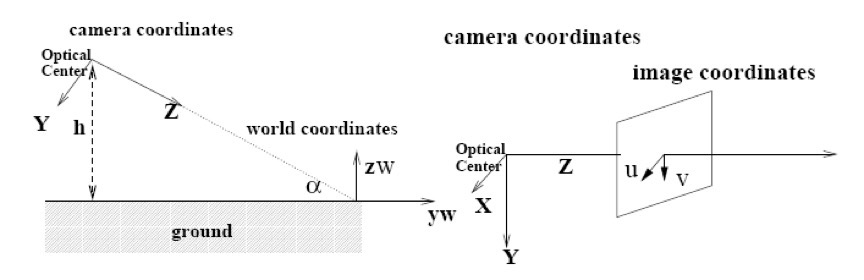
\includegraphics[width=0.7\linewidth]{coord.jpg}
    \caption{Coordinate System}
    \end{figure}
    \begin{solution}
        First of all, find the rotation matrix $R$ that maps points in world coordinate to the same points in camera coordinate. Since the rotation is about $x$ axis, it can be described by the matrix ($\theta$ is defined using right-hand rule):
        
        \begin{equation}
            \begin{split}
            R _ { x } ( \theta )
            & = \left[ \begin{array} { c c c } { 1 } & { 0 } & { 0 } \\ { 0 } & { \cos \theta } & { - \sin \theta } \\ { 0 } & { \sin \theta } & { \cos \theta } \end{array} \right] \\
            & = \left[ \begin{array} { c c c } { 1 } & { 0 } & { 0 } \\ { 0 } & { - \sin \alpha } & { - \cos \alpha } \\ { 0 } & { \cos \alpha } & { - \sin \alpha } \end{array} \right], \ \theta = \frac{\pi}{2} + \alpha 
        \end{split}
        \end{equation}
        
        Next, the translation vector is defined by the world origin expressed in the camera frame:
        \[ t = \left( \begin{array} {c} {0} \\ {0} \\ {\frac{h}{\sin \alpha}} \\ \end{array} \right) \]
        
        Composite the Euclidean transformation described in Eq. (2) and the perspective projection described in Eq. (1):
        \[ 
        \begin{split}
            M 
            &= \left[ \begin{array} { l l l l } { f } & { 0 } & { 0 } & { 0 } \\ { 0 } & { f } & { 0 } & { 0 } \\ { 0 } & { 0 } & { 1 } & { 0 } \end{array} \right] \left[ \begin{array} { c c c c } { 1 } & { 0 } & { 0 } & { 0 } \\ { 0 } & { - \sin \alpha } & { - \cos \alpha } & { 0 } \\ { 0 } & { \cos \alpha } & { - \sin \alpha } & { \frac{h}{\sin \alpha} } \\ { 0 } & { 0 } & { 0 } & { 1 } \end{array} \right] \\
            &= \left[ \begin{array} { l l l l } { f } & { 0 } & { 0 } & { 0 } \\ { 0 } & { -f\sin\alpha } & { -f\cos\alpha } & { 0 } \\ { 0 } & { \cos \alpha } & { -\sin \alpha } & { \frac{h}{\sin \alpha} } \end{array} \right] \\
        \end{split}
        \]
    With this, 
    \end{solution}
    
    \subpart
    * Find the $3 \times 3$ matrix for the linear transformation that maps points on the world plane $Z_w = d$ to the image plane $(u, v, w)$.
    \begin{solution}
        Borrowing the result from part (ii):
        \[
        \begin{split}
        \left( \begin{array} { c } { u } \\ { v } \\ { w } \end{array} \right) 
        &= M \left( \begin{array} { c } { X _ { w } } \\ { Y _ { w } } \\ { Z _ { w } } \\ { 1 } \end{array} \right) \\
        &= \left[ \begin{array} { l l l l } { f } & { 0 } & { 0 } & { 0 } \\ { 0 } & { -f\sin\alpha } & { -f\cos\alpha } & { 0 } \\ { 0 } & { \cos \alpha } & { -\sin \alpha } & { \frac{h}{\sin \alpha} } \end{array} \right] \left( \begin{array} { c } { X _ { w } } \\ { Y _ { w } } \\ { d } \\ { 1 } \end{array} \right) \\
        &= \left( \begin{array} { c } { f X _ { w } } \\ { - f Y _ { w } \sin \alpha - f d \cos \alpha } \\ { Y _ { w } \cos \alpha - d \sin \alpha + \frac{h}{\sin \alpha} } \end{array} \right) \\
        \end{split}
        \]
    We need to convert this into a $M ^ {'} _ {3 \times 3} \left( \begin{array} {c} X _ {w} \\ Y _ {w} \\ 1 \\ \end{array} \right)$ form:
    \[  \left( \begin{array} { c } { u } \\ { v } \\ { w }            \end{array} \right) = \begin{bmatrix}
        f & 0 & 0 \\
        0 & -f\sin \alpha & -fd \cos \alpha \\
        0 & \cos \alpha & \frac{h}{\sin \alpha} - d \sin \alpha \\
        \end{bmatrix}
        \left( \begin{array} {c} {X _ {w}} \\ {Y _ {w}} \\ {1} \\ \end{array} \right) \\
    \]

    \end{solution}
\end{subparts}


\end{parts}
\end{questions}